%-------------------------------------------------------------------------------
\section{Evaluation}
%-------------------------------------------------------------------------------
For our evaluation, we obtained traces from a large e-commerce company, where the underlying system is a micro-service architecture. The traces encapsulate the request-response interactions of micro-services. We obtained traces from three request paths in the system that correspond to viewing, selling and checking out an item in the catalog. The request paths are not mutually exclusive i.e. they share some services\kam{TODO: How many shared services?} and traces from the same request path can vary subtly based on the exact request parameters. We use graphs corresponding to a small fraction of traces are used to generate node embeddings. As mentioned in the previous section\kam{Use section labels?}, we compute trace embeddings by aggregating node embeddings. In particular, for every trace, we sum the node embeddings of the nodes present in the trace to obtain the corresponding graph embedding. Since the process of generating node embeddings involves random walks in the graph as well as tuning hyper-parameters, we generate node embeddings several (< 10) times. In each instance, we compute the corresponding trace embeddings. 

%Since clustering of traces based on execution paths depends on graph structure, it serves as the reference task. Trace embeddings that perform best on clustering ate used for other downstream tasks such as classification and fault diagnostics.  
\kam{TODO: How many traces are used to generate node embeddings? We currently use 200 traces to learn embeddings, and the total number of traces is ~4500. We haven't yet verified how many of these traces are duplicates.}
  
\subsection{Clustering}
 Clustering traces by execution paths can be used to determine the number of distinctive request paths as well as to be able to easily produce examples of successful executions of the system executing a particular request path. The computed trace embeddings represent points in $R^{d}$ space, for which we obtain clusters using the K-means approach, with K = 3. 
 
 \kam{\textbf{MUST-TRY}If we swept the value for K, find the K for which the clusters are most stable and then compare predicted values to expected values, this will allow us to say that we can determine the number of distinctive request paths. This is a useful contribution so long as request paths are not mutually exclusive.}
 
 \begin{figure}
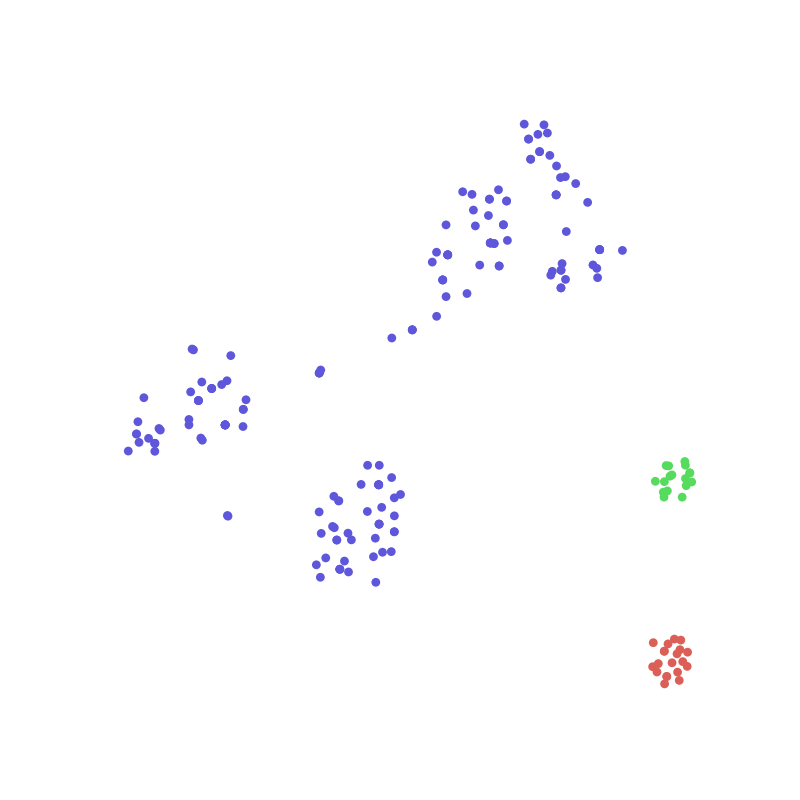
\includegraphics[scale=0.2]{tsne_viz.png}
\caption{2-D representation of clusters learned by K-means with graph embeddings as input}
\label{Clusters}
\end{figure}
 
Since we know the labels for the traces a priori, we can compute the Agjusted-Rand\kam{may need to cite} measure, which is a bounded value between [-1,1], where 0 or negative values indicate that the data points were drawn randomly and 1 is the perfect score. \kam{Consider computing number of false positives and false negatives instead. Gives us better interpretability} Trace embeddings which performed best returned a perfect score. The high dimensional data points are projected to 2-D using t-SNE and distinctive clusters can be seen in figure. Though we are able to learn clusters based on the data accurately, there is a large spread within individual clusters, which translates to poor results for predictive analysis. That is to say, predicting which cluster a new trace belongs to returns inaccurate results for a significant percentage of cases\kam{Need to quantify significant. I think it is more than 50\%, but I don't recall off hand}

\kam{\textbf{MUSTDO}: Draw traces from more than three execution paths. Not only will that add credibility, we also expect to show that the clusters of families of traces that share more services are closer than other clusters. Steps} \newline
\kam{
\begin{enumerate}
\item Pull traces from different request paths from production
\item Since tracing can return too few nodes, determine the minimum number of nodes which should be present in a trace for us to include the trace. Does this need to be a path specific or agnostic?
\item Given a bunch of traces to consider, weed out the duplicates
\item Now randomly shuffle the graphs and learn node representations. Aggregate to obtain trace embeddings. 
\item Cluster the embeddings using K-means. Since we know the labels for each of the traces a priori, we can compute an adjusted-rand measure, which is a bounded value between [-1,1], with 1 being the perfect score. 
\item With NodeCount as graph representation, what is the best value of adjusted rand measure? Number of false positives and false negatives?
\end{enumerate}
} \newline
\kam{Expectation: Graph embeddings performs better than NodeCount. This is the result we saw in the experiment we ran, but that was only one experiment} \newline
\kam{Plot the number of false positives and false negatives for the two approaches as the corpus of traces increases in size. We expect embeddings to perform objectively better than graphKernels and numbers to grow as the size of corpus increases and then level off} \newline

\kam{\textbf{SHOULD DO} \newline Randomization} \newline
\kam{Steps: \newline
\begin{enumerate}
\item Subtractive randomness: Some number of spans may be missing in a number of traces, which we are dubbing subtractive randomness. Is this signifiant enough to impact our baseline performance? Am how do embeddings perform? The expected result here is that the performance of embeddings stays near constant, while that of our baseline deteriorates proportional to the degree of randomness. We only want to include this graph if the deterioration is noticeable.
\item Additive randomness: Add random noise into the traces, such that there are a few nodes in each trace. Is this realistic? 
\item Additive + Subtractive randomness
\end{enumerate}
} 

\kam{\textbf{TODO: Exploratory}\newline XTrace data (old and new)\newline
The embeddings will not learn different clusters unless the DAG of executions are structurally different. So far, the XTrace data does not look significantly different and embeddings perform poorly on these. Work in progress.
}

\kam{\textbf{TODO: Exploratory}\newline Clustering on Uber graphs)\newline
Need to clean up code base and write code for parsing and processing data based on the snippet that Jonathan sent me. Work in progress.
}

\subsection{Classification}
Given a new trace, a user may wish to know which family the new trace belongs to. If we observed a set of executions and knew their labels, the scenario described is the perfect use case for classification. We split our graphs into a training set and test set and are able to learn a logistic regression classifier that is able to predict the class of any test graph with accuracy close to 100\%, as can be seen in Figure~\ref{Classification}. Classification works near-perfectly even when the number of dimensions for node embeddings is as low as 4.

\begin{figure}
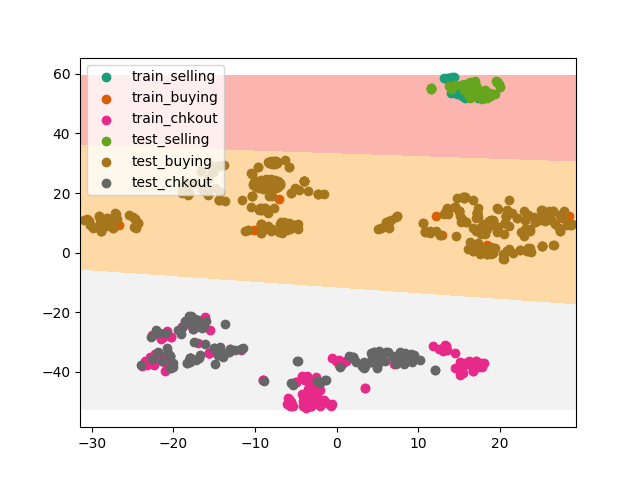
\includegraphics[scale=0.5]{test_logistic_2d.png}
\caption{Logistic regression}
\label{Classification}
\end{figure}

\kam{\textbf{MUSTDO} \newline The classification was setup to classify graphs of failed traces and was learning on graphs of successful traces. Apart from the fact that our criteria for failed and successful traces need to be revisited, we might want to set this problem up slightly differently. Set up k-fold cross-validation with k=10. }\newline
\kam{Expected result: Performance of classification keeps getting better as we increase k. Try for values of k = 5,10,15,20,25. If the performance is noticeably different, we can plot a graph for precision and recall of classifier.}

\subsection{Automated Fault diagnostics}
In section 2, we presented the call graph of a trace from a failed execution obtained during an outage. In the call graph, multiple services were alerting due to downstream failures and that the SRE deems the possible cause of failure to be downstream service(s) not being called. The next step for the SRE is to difference the call graph for the failed execution with those of the successful execution(s). With trace embeddings, we compute the pairwise euclidean distance of the trace embedding from the failed execution with that of every observed successful execution exercising the same request path. In so doing, we avoid computing more conventional distance measures such as graph edit distance, which has been shown to be NP-complete. 

\begin{figure}
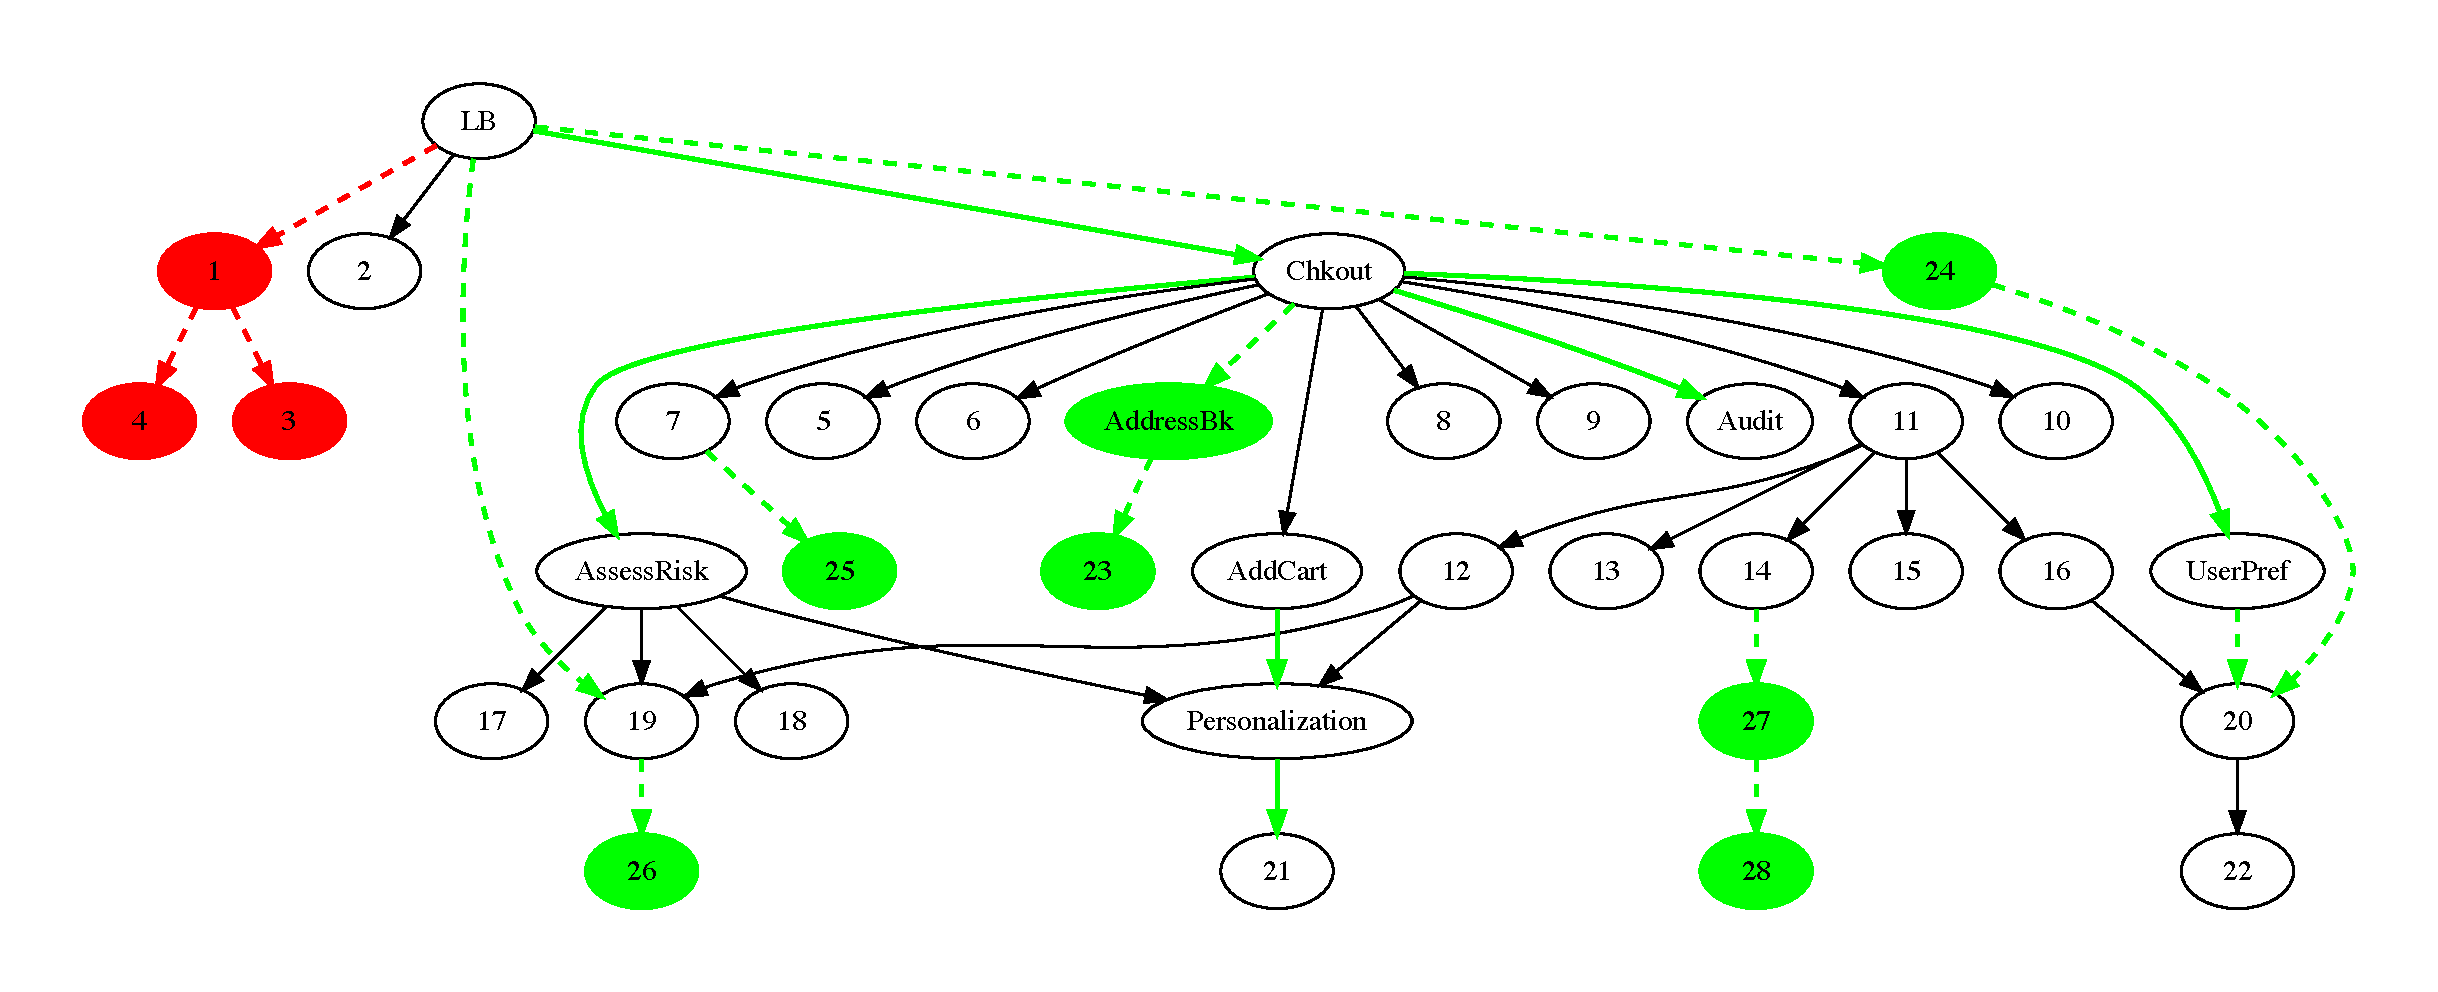
\includegraphics[width=0.5\textwidth]{anon_adrbk_repair.pdf}
\caption{Services to be added are in solid green, those to be deleted in solid red. Edges to be added are in dashed green, those to be deleted are in dashed red. Solid green edges represent status needs to be successful instead of failed. TODO: This is an older repair image, needs to be updated. }
\label{RootCauseHint}
\end{figure}

Figure~\ref{RootCauseHint} demonstrates the additions and deletions suggested to the original call graph that would make this interaction successful, in this case, a successful checkout. Of the two possible services which might have been the cause of failure, we can very quickly establish that service 1 and 24 are aliases of each other and therefore, the only hint to investigate further is AddressBk service. And it turns out that the user was unable to purchase items from the store as a result of the AddressBook service being down. 

\kam{Investigate: Some completions are worse than others. Why? For most cases, if we did compute graph edit distance, we would get the best results. Results obtained from representations are slightly off. But in 1 out of the 5 cases, the result appears to be really off. Maybe the corpus is too small?} \newline

\kam{TODO: Distinguish between failed and successful executions in different domains. When we obtain traces from production, we may also need to do some work to determine if the traces was successful or not.  This may involve calling out to external data sources.}\newline

\kam{\textbf{SHOULD DO}\newline Failed executions from injected faults. Steps} \newline
\kam{
\begin{itemize}
\item For e2e tests in checkout, inject faults taking down the mandatory services one at a time to obtain call graphs for failed executions for multiple request paths. 
\item Run viewitem test and inject faults in mandatory services for viewitem as well. 
\item Compute trace embeddings for the traces collected.
\item Filter successful traces so that for each trace drawn from a failed execution, it is only compared to successful traces exercising the same request path. 
\item For each failed execution, find the closest successful execution i.e. the one with the minimum euclidean distance. 
\item Compute the graph edit distance of the trace as determined by our technique and compare it to the minimal graph edit distance
\end{itemize}
}

\kam{\textbf{COULD DO} \newline Collect real outage data from looking at eBay's JIRA. Steps} \newline
\kam{
\begin{enumerate}
\item For every outage in the last 90 days, is this an outage we can potentially fix?
\item For every outage we can potentially fix, can we produce the outage using a test and injected faults?
\item Given a trace of an outage, does the repair suggested point to its root cause?
\item Can we quantify how long it takes us to suggest a hint as opposed to amount of time that was spent on the issue?
\end{enumerate}
}
\kam{Results we want to report: \newline
\begin{enumerate}
\item Percentage of total outages we can provide hints for
\item Of the outages we can provide hints for, present overall time taken by our technique to provide hint v/s time spent triaging the outage
\item Ballpark figures of revenue costs associated with the outages that we might have been able to help with
\end{enumerate}
}

\kam{\textbf{COULD DO} \newline As we have described above, we need to compute pairwise distance of a trace from a failed execution to all successful executions exercising the same request path. While we avoid computing graph edit distance, we also don't want to compare with EVERY successful execution exercising the same request path. If we are able to separate graphs of failed executions from successful executions, then we can compare only with a few canonical graphs of successful executions.} \newline

\kam{\textbf{Will not do now} \newline Can we re-construct graphs from embeddings? Information loss? This is more of a research question. How much information do we lose from throwing away traces? What does this mean in terms of recovering the graph from the embedding? } \newline
\kam{\textbf{Will not do now} \newline Using a different aggregator? This is a more long term goal. It is a good  idea to compare with a different aggregator just to see how each performs. But more importantly, if there is too much information loss with summation, we may not be able to re-generate the graph from the embedding. What aggregator will allow us to recover graph from embedding? And what are its applications to graph generation? } \newline

\kam{Sum up the eval}



















